\chapter{Periodicity}\label{ch:b1:periodicity}

Lithium, sodium and potassium are soft, shiny metals that tarnish in air
and react with water; fluorine, chlorine and bromine are coloured,
corrosive non-metals that snatch electrons from almost anything. Each
trio sits in one column of the periodic table, and the members of a
column resemble one another while neighbours along a row do not. The
previous chapter explained why: elements of one column have the same
configuration of \omterm{def:b1:quantum-numbers:configuration}{valence electrons}. This chapter turns that explanation
into numbers --- radii, ionisation energies, electron affinities,
electronegativities --- and into the trends that let a chemist predict,
from the position of an element alone, how large its atoms are, how
easily they give up or accept electrons, and which way the electrons of
a bond lean.

\begin{recall}
Every \omterm{def:b1:periodicity:table}{period} begins with the filling of an $n$s \omterm{def:b1:quantum-numbers:orbital}{subshell} and ends with a
filled $n$p \omterm{def:b1:quantum-numbers:orbital}{subshell}; the s, p, d and f \omterm{def:b1:periodicity:table}{blocks} have the widths 2, 6, 10
and 14 (\cref{prop:b1:quantum-numbers:table}). Book 1 (grade 11)
described \omterm{def:b1:periodicity:electronegativity}{electronegativity} as the tendency of an atom to attract the
electrons of a bond.
\end{recall}

\section{The table built from configurations}

\begin{definition}[Period, group, block]\label{def:b1:periodicity:table}
In the periodic table the elements are listed by increasing atomic
number $Z$. A \emph{period}\index{period} is a row: the elements whose
valence shell has the same principal number $n$. A
\emph{group}\index{group} is a column, numbered 1 to 18: the elements
with the same valence configuration. A \emph{block}\index{block} is the
set of elements whose last-filled \omterm{def:b1:quantum-numbers:orbital}{subshell} is of one kind, s, p, d or f.
\end{definition}

\begin{example}[Reading a position]\label{ex:b1:periodicity:position}
Selenium, $[\ce{Ar}]\,3\text{d}^{10} 4\text{s}^2 4\text{p}^4$, is in
\omterm{def:b1:periodicity:table}{period} 4 (valence shell $n = 4$), in the p \omterm{def:b1:periodicity:table}{block}, and in \omterm{def:b1:periodicity:table}{group} 16 (two s
electrons, ten d and four p: $2 + 10 + 4$); its valence configuration
$n\text{s}^2 n\text{p}^4$ is that of oxygen and sulfur above it.
\end{example}

\begin{definition}[Metal, non-metal, metalloid]\label{def:b1:periodicity:metalloid}
A metal is an element whose solid conducts electricity and whose atoms
readily lose electrons to form cations; a non-metal is an element that
does not conduct (with exceptions such as graphite) and readily gains
electrons or shares them. A \emph{metalloid}\index{metalloid} is an
element of intermediate character, a semiconductor: boron, silicon,
germanium, arsenic, antimony and tellurium.
\end{definition}

\begin{omfigure}
\omperiodictable[colour=metals, legend, f block=false]

{\small Metals (the great majority), \omterm{def:b1:periodicity:metalloid}{metalloids} along a staircase from
boron to tellurium, and non-metals in the upper right. The f \omterm{def:b1:periodicity:table}{block},
omitted here, is made of metals.}
\end{omfigure}

\section{Size: atomic and ionic radii}

\begin{definition}[Screening, effective nuclear charge]\label{def:b1:periodicity:screening}
In an atom with several electrons, an electron is attracted by the
nucleus, of charge $Ze$, and repelled by the other electrons. The inner
electrons partly cancel the attraction of the nucleus: this is
\emph{screening}\index{screening}. The valence electron behaves as if it
felt a reduced nuclear charge $Z^{*}e$, the \emph{effective nuclear
charge}\index{effective nuclear charge}, with $Z^{*} < Z$. Electrons of
an inner shell screen almost completely; electrons of the same shell
screen only a little.
\end{definition}

\begin{remark}[A qualitative tool]\label{rem:b1:periodicity:slater}
In this book $Z^{*}$ is used qualitatively: along a \omterm{def:b1:periodicity:table}{period}, $Z$
increases by one at each step while the added electron, in the same
shell, screens only a little, so $Z^{*}$ felt by the \omterm{def:b1:quantum-numbers:configuration}{valence electrons}
increases; down a group, $Z^{*}$ changes little but the valence shell
$n$ grows. Rules to compute $Z^{*}$ from the configuration (Slater's
rules) are given in the Year 2 volume.
\end{remark}

\begin{definition}[Covalent radius, ionic radius]\label{def:b1:periodicity:radius}
The \emph{covalent radius}\index{covalent radius} of an element is half
the length of a single bond between two of its atoms: for chlorine, half
the \ce{Cl-Cl} distance of \ce{Cl2}. The \emph{ionic
radius}\index{ionic radius} of an ion is the share of the distance
between neighbouring cations and anions in ionic crystals attributed to
it, from a convention that fixes the radius of one reference ion
(\ce{O^{2-}}); it depends slightly on the number of neighbours.
\end{definition}

\begin{example}[The halogens]\label{ex:b1:periodicity:halogen-radii}
The bond lengths of \ce{F2}, \ce{Cl2}, \ce{Br2} and \ce{I2} are 141.2,
198.8, 228.1 and \qty{266.6}{pm}, so the covalent radii are 71, 99, 114
and \qty{133}{pm}: each step down the group adds a shell and about
\qty{20}{pm} or more.
% ledger: re:F2, re:Cl2, re:Br2, re:I2
\end{example}

\begin{proposition}[Trends in radius]\label{prop:b1:periodicity:radius-trend}
Atomic radii decrease from left to right along a \omterm{def:b1:periodicity:table}{period} and increase
from top to bottom down a group. A cation is smaller than its atom, an
anion larger; in an isoelectronic series (ions with the same
configuration) the radius decreases as $Z$ increases.
\end{proposition}

\begin{proof}[Reasoning]
The size of an atom is the size of its valence orbitals, which shrink
when $Z^{*}$ grows and swell when $n$ grows. Along a \omterm{def:b1:periodicity:table}{period} $n$ is fixed
and $Z^{*}$ grows: the atoms contract. Down a group $n$ grows by one at
each step, which outweighs the small change of $Z^{*}$. A cation has lost
its valence shell, or electrons that repelled one another; an anion has
gained an electron that repels the others. In an isoelectronic series
the same electrons are held by a nucleus of growing charge.
\end{proof}

\begin{omfigure}
\begin{tikzpicture}[font=\small, x=1pt, y=1pt]
  % ledger: rion:O2-VI, rion:F-VI, rion:Na+VI, rion:Mg2+VI, rion:Al3+VI
  % radii in pm drawn at 0.30 pt per pm (circles to scale)
  \foreach \x/\r/\lab/\v in {40/140/\ce{O^{2-}}/140, 130/133/\ce{F-}/133,
      210/102/\ce{Na+}/102, 275/72/\ce{Mg^{2+}}/72, 325/53.5/\ce{Al^{3+}}/54} {
    \draw[fill=omDef!20, draw=omDef!70!black] (\x,0) circle ({0.30*\r});
    \node at (\x,0) {\lab};
    \node[below] at (\x,-50) {\v\,pm};
  }
  \node[anchor=west, align=left] at (350,0) {ten electrons each,\\$Z = 8 \to 13$};
\end{tikzpicture}

{\small The isoelectronic series $1\text{s}^2 2\text{s}^2 2\text{p}^6$,
drawn to scale (ionic radii for six neighbours). The same ten electrons
shrink as the nuclear charge grows.}
\end{omfigure}

\section{Energies: ionisation and electron affinity}

\begin{definition}[Ionisation energies]\label{def:b1:periodicity:ionisation-energy}
The \emph{first ionisation energy}\index{first ionisation energy} $E_{i1}$
of an element is the energy needed to remove one electron from the
isolated atom in its \omterm{def:b1:quantum-numbers:energy-level}{ground state}, in the gas phase:
\[
  \ce{X(g) -> X+(g) + e-}, \qquad E_{i1} = E(\ce{X+}) + E(\ce{e-}) - E(\ce{X}) > 0 .
\]
The \emph{successive ionisation energies}\index{successive ionisation
energies} $E_{i2}, E_{i3}, \dots$ remove the second, the third
electron\dots\ from \ce{X+}, \ce{X^{2+}}\dots\ They are given in
electronvolts per atom or in kilojoules per mole
($\qty{1}{eV} \leftrightarrow \qty{96.49}{kJ/mol}$).
% ledger: const:NA, const:e (1 eV x N_A = 96.485 kJ/mol)
\end{definition}

\begin{omfigure}
\begin{tikzpicture}
\begin{axis}[
  width=0.92\linewidth, height=6.4cm,
  xmin=0, xmax=37, ymin=0, ymax=27,
  axis x line=bottom, axis y line=left,
  xlabel={atomic number $Z$}, ylabel={$E_{i1}$ (eV)},
  xtick={2,10,18,36}, ytick={0,5,10,15,20,25},
  tick label style={font=\small}, label style={font=\small},
  clip=false]
\addplot[omDef, thick, mark=*, mark size=1.3pt] table[x=Z, y=IE_eV] {figdata/out/bachelor-1-ionisation-energies.dat};
\node[font=\small, anchor=south] at (axis cs:2,24.6) {He};
\node[font=\small, anchor=south] at (axis cs:10,21.6) {Ne};
\node[font=\small, anchor=south] at (axis cs:18,15.8) {Ar};
\node[font=\small, anchor=south] at (axis cs:36,14.0) {Kr};
\node[font=\small, anchor=north] at (axis cs:3,5.2) {Li};
\node[font=\small, anchor=north] at (axis cs:11,4.9) {Na};
\node[font=\small, anchor=north] at (axis cs:19,4.1) {K};
\node[font=\small, anchor=north] at (axis cs:31,5.8) {Ga};
\node[font=\small, anchor=north] at (axis cs:5,7.9) {B};
\node[font=\small, anchor=north] at (axis cs:8,13.2) {O};
\node[font=\small, anchor=north west] at (axis cs:13.1,6.0) {Al};
\node[font=\small, anchor=north] at (axis cs:16,9.9) {S};
\node[font=\small, anchor=south] at (axis cs:26,8.0) {3d metals};
\end{axis}
\end{tikzpicture}

{\small First ionisation energies of the first 36 elements. Maxima at the
noble gases, minima at the alkali metals; the small dips at B, Al, Ga
and at O, S are the \omterm{def:b1:quantum-numbers:orbital}{subshell} effects of
\cref{prop:b1:periodicity:ie-anomalies}.}
\end{omfigure}

\begin{proposition}[Trends in ionisation energy]\label{prop:b1:periodicity:ie-trend}
The \omterm{def:b1:periodicity:ionisation-energy}{first ionisation energy} increases along a \omterm{def:b1:periodicity:table}{period}, from the alkali
metal to the noble gas, and decreases down a group. \omterm{def:b1:periodicity:ionisation-energy}{Successive
ionisation energies} always increase, $E_{i1} < E_{i2} < \dots$, and jump
by a large factor when the electron removed belongs to an inner shell.
\end{proposition}

\begin{proof}[Reasoning]
Removing an electron is easier when it is far from the nucleus and feels
a small $Z^{*}$: along a \omterm{def:b1:periodicity:table}{period} $Z^{*}$ grows and the radius shrinks; down
a group the radius grows. Each successive electron is pulled from an ion
of higher charge and smaller size, so costs more; once the valence shell
is empty the next electron comes from a shell of smaller $n$, much closer
to the nucleus and hardly screened at all.
\end{proof}

\begin{example}[Magnesium]\label{ex:b1:periodicity:magnesium}
The \omterm{def:b1:periodicity:ionisation-energy}{successive ionisation energies} of magnesium are 7.65, 15.04, 80.14
and \qty{109.27}{eV}. The ratio $E_{i2}/E_{i1} \approx 2$ is moderate;
$E_{i3}/E_{i2} \approx 5.3$ is a jump: the third electron comes from the
2p core. Magnesium gives up its two 3s electrons and stops at
\ce{Mg^{2+}}, the noble-gas configuration of neon.
% ledger: ie:Mg, ie2:Mg, ie3:Mg, ie4:Mg
\end{example}

\begin{omfigure}
\begin{tikzpicture}
\begin{axis}[
  width=0.55\linewidth, height=5.2cm, ybar, bar width=14pt,
  xmin=0.4, xmax=4.6, ymin=1, ymax=300, ymode=log,
  axis x line=bottom, axis y line=left,
  xlabel={electron removed}, ylabel={$E_{i}$ (eV)},
  xtick={1,2,3,4}, xticklabels={1st,2nd,3rd,4th},
  tick label style={font=\small}, label style={font=\small},
  nodes near coords={\pgfmathprintnumber[fixed, fixed zerofill, precision=2]{\pgfplotspointmeta}},
  nodes near coords style={font=\scriptsize},
  point meta=rawy]
\addplot[fill=omDef!40, draw=omDef] table[x=k, y=IE_eV] {figdata/out/bachelor-1-ionisation-energies-mg.dat};
\end{axis}
\end{tikzpicture}

{\small \omterm{def:b1:periodicity:ionisation-energy}{Successive ionisation energies} of magnesium (logarithmic axis).
The third is five times the second: the 3s shell is empty and the core
is reached.}
\end{omfigure}

\begin{proposition}[Two dips along a period]\label{prop:b1:periodicity:ie-anomalies}
Along \omterm{def:b1:periodicity:table}{periods} 2 and 3, the \omterm{def:b1:periodicity:ionisation-energy}{first ionisation energy} drops slightly from
\omterm{def:b1:periodicity:table}{group} 2 to \omterm{def:b1:periodicity:table}{group} 13 (\ce{Be} to \ce{B}, \ce{Mg} to \ce{Al}) and from
\omterm{def:b1:periodicity:table}{group} 15 to \omterm{def:b1:periodicity:table}{group} 16 (\ce{N} to \ce{O}, \ce{P} to \ce{S}).
\end{proposition}

\begin{proof}[Reasoning]
In \ce{B} and \ce{Al} the electron removed is the first p electron,
higher in energy than the s electrons of \ce{Be} and \ce{Mg}. In \ce{O}
and \ce{S} the electron removed is the fourth p electron, the first to
share an orbital (\omorbs{ud,u,u}): its repulsion with its partner makes
it easier to remove than an electron of the half-filled \omterm{def:b1:quantum-numbers:orbital}{subshell} of
\ce{N} or \ce{P} (\omorbs{u,u,u}).
% ledger: ie:Be, ie:B, ie:N, ie:O, ie:Mg, ie:Al, ie:P, ie:S
\end{proof}

\begin{definition}[Electron affinity]\label{def:b1:periodicity:electron-affinity}
The \emph{electron affinity}\index{electron affinity} $E_{ea}$ of an
element is the energy released when an isolated atom in its \omterm{def:b1:quantum-numbers:energy-level}{ground state}
captures an electron in the gas phase,
\[
  \ce{X(g) + e- -> X-(g)}, \qquad E_{ea} = E(\ce{X}) + E(\ce{e-}) - E(\ce{X-}) .
\]
It is positive when the anion is more stable than the atom and the free
electron.
\end{definition}

\begin{example}[Halogens and their neighbours]\label{ex:b1:periodicity:ea}
The electron affinities of \ce{F}, \ce{Cl}, \ce{Br} and \ce{I} are 3.40,
3.61, 3.36 and \qty{3.06}{eV}, the largest of all elements; those of
\ce{O} and \ce{S} are 1.44 and \qty{2.02}{eV}, of \ce{C} \qty{1.26}{eV},
of \ce{Na} \qty{0.55}{eV}. Atoms that complete a \omterm{def:b1:quantum-numbers:orbital}{subshell} by capturing
an electron (the halogens) release much energy. Nitrogen, beryllium,
magnesium and the noble gases form no stable gaseous anion: the extra
electron would have to pair in a half-filled p \omterm{def:b1:quantum-numbers:orbital}{subshell} or enter a new
\omterm{def:b1:quantum-numbers:orbital}{subshell}. Fluorine's affinity is smaller than chlorine's because the
added electron is crowded into the small 2p shell.
% ledger: ea:F, ea:Cl, ea:Br, ea:I, ea:O, ea:S, ea:C, ea:Na
\end{example}

\section{Electronegativity and polarisability}

\begin{definition}[Electronegativity]\label{def:b1:periodicity:electronegativity}
The \emph{electronegativity}\index{electronegativity} $\chi$ of an
element measures the tendency of its atoms, in a molecule, to attract
the electrons of the bonds they form. Two scales are in use.
\begin{itemize}
  \item On the \emph{Pauling scale}\index{Pauling scale}, differences
        are defined from bond energies $D$:
        \[
          |\chi_A - \chi_B| = \sqrt{\frac{\Delta E}{\qty{1}{eV}}}, \qquad
          \Delta E = D(\text{A--B}) - \tfrac12\big[D(\text{A--A}) +
          D(\text{B--B})\big],
        \]
        and the scale is anchored by $\chi(\ce{F}) = 3.98$.
  \item On the \emph{Mulliken scale}\index{Mulliken scale},
        $\chi_M = \tfrac12\,(E_{i1} + E_{ea})$, in electronvolts.
\end{itemize}
\end{definition}

\begin{remark}[Why the extra bond energy]\label{rem:b1:periodicity:pauling}
If the two atoms of a bond A--B attracted its electrons equally, the bond
energy would be about the average of those of A--A and B--B. When one
atom is more electronegative, the bond acquires a partial ionic
character, $\ce{A^{\delta+}-B^{\delta-}}$, whose electrostatic attraction
adds energy: $\Delta E > 0$ measures the unequal sharing. The Mulliken
definition says the same thing from the atoms' side: an atom that holds
its own electrons tightly ($E_i$ large) and welcomes an extra one
($E_{ea}$ large) attracts the electrons of a bond.
\end{remark}

\begin{omfigure}
% ledger: en:H, en:Li, en:Be, en:B, en:C, en:N, en:O, en:F, en:Na, en:Mg,
% en:Al, en:Si, en:P, en:S, en:Cl, en:K, en:Ca, en:Ga, en:Ge, en:As, en:Se,
% en:Br, en:Rb, en:Sr, en:In, en:Sn, en:Sb, en:Te, en:I, en:Cs, en:Ba
\omperiodictable[upto=56, f block=false, numbers=false, highlight colour=omDef!12,
  highlight={F,O,N,Cl}, values={H/2.20,Li/0.98,Be/1.57,B/2.04,C/2.55,N/3.04,O/3.44,F/3.98,
  Na/0.93,Mg/1.31,Al/1.61,Si/1.90,P/2.19,S/2.58,Cl/3.16,K/0.82,Ca/1.00,Ga/1.81,Ge/2.01,
  As/2.18,Se/2.55,Br/2.96,Rb/0.82,Sr/0.95,In/1.78,Sn/1.96,Sb/2.05,Te/2.10,I/2.66,
  Cs/0.79,Ba/0.89}]

{\small Pauling electronegativities of the main-group elements (the d
\omterm{def:b1:periodicity:table}{block} is left blank). They increase from left to right and from bottom to
top; the four most electronegative elements, F, O, Cl and N, are shaded.}
\end{omfigure}

\begin{proposition}[Trends in electronegativity]\label{prop:b1:periodicity:en-trend}
\omterm{def:b1:periodicity:electronegativity}{Electronegativity} increases along a \omterm{def:b1:periodicity:table}{period} and decreases down a group:
fluorine is the most electronegative element, caesium and francium the
least. The difference $\Delta\chi$ between two bonded atoms gives the
character of the bond: $\Delta\chi < 0.4$ nearly non-polar covalent,
$0.4 < \Delta\chi < 1.7$ polar covalent, $\Delta\chi > 1.7$ mainly ionic
--- three regions of a continuum, not sharp classes.
\end{proposition}

\begin{example}[Three bonds]\label{ex:b1:periodicity:bonds}
\ce{C-H}: $\Delta\chi = 2.55 - 2.20 = 0.35$, nearly non-polar;
\ce{O-H}: $3.44 - 2.20 = 1.24$, polar, the oxygen carrying a partial
negative charge; \ce{Na-Cl}: $3.16 - 0.93 = 2.23$, ionic.
% ledger: en:C, en:H, en:O, en:Na, en:Cl
\end{example}

\begin{definition}[Polarisability]\label{def:b1:periodicity:polarisability}
The \emph{polarisability}\index{polarisability} of an atom, ion or
molecule measures how easily its electron cloud is deformed by an
electric field --- the field of a neighbouring ion or dipole. A
polarisable species acquires, in a field, an induced dipole moment
proportional to the field.
\end{definition}

\begin{proposition}[Trends in polarisability]\label{prop:b1:periodicity:polarisability-trend}
\omterm{def:b1:periodicity:polarisability}{Polarisability} grows with the size of the electron cloud and with the
number of electrons, and decreases with the charge of the nucleus that
holds them: it increases down a group ($\ce{F-} < \ce{Cl-} < \ce{Br-} <
\ce{I-}$), anions are much more polarisable than cations, and large
soft anions such as \ce{I-} are the most polarisable common species.
\end{proposition}

\begin{example}[Why polarisability matters]\label{ex:b1:periodicity:pol}
The London attraction between molecules, the subject of
\cref{ch:b1:intermolecular-forces-solvents}, grows with \omterm{def:b1:periodicity:polarisability}{polarisability}:
diiodine is a solid at room temperature, dichlorine a gas. In an ionic
crystal, a small highly charged cation polarises a large anion and gives
the bond some covalent character, the failure of the simple ionic model
met in \cref{ch:b1:crystals-ionic-covalent}.
\end{example}

\begin{history}[Pauling's scale, 1932]
In 1932 the American chemist Linus Pauling noticed that the energy of a
bond between two different atoms is almost always larger than the
average of the energies of the two symmetric bonds, and built from that
excess the first scale of \omterm{def:b1:periodicity:electronegativity}{electronegativity}. Revised as better bond
energies were measured, his scale is still the one in every table.
Pauling received the Nobel Prize in Chemistry in 1954, for his work on
the chemical bond, and the Nobel Peace Prize in 1962.
\end{history}

\begin{omfigure}
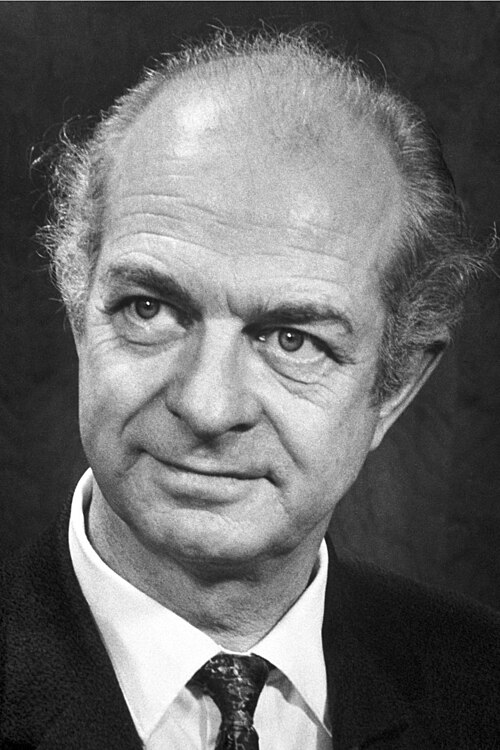
\includegraphics[width=0.24\linewidth]{images/book2/pauling.jpg}

{\small Linus Pauling (1901--1994).}
\end{omfigure}

\section{Trends in chemical character}

\begin{proposition}[Reducing and oxidising character]\label{prop:b1:periodicity:redox-trend}
Elements of low ionisation energy and low \omterm{def:b1:periodicity:electronegativity}{electronegativity}, on the left
of the table and at the bottom of their groups, readily lose electrons:
they are reducing metals (the alkali metals most of all). Elements of
high \omterm{def:b1:periodicity:electronegativity}{electronegativity} and \omterm{def:b1:periodicity:electron-affinity}{electron affinity}, in the upper right, readily
gain electrons: they are oxidising non-metals (fluorine, oxygen and
chlorine most of all). The noble gases, with a high ionisation energy and
no affinity for an extra electron, do neither.
\end{proposition}

\begin{method}[Predicting a trend from the position]\label{met:b1:periodicity:predict}
To compare two elements for a property tied to the hold of the nucleus
on the \omterm{def:b1:quantum-numbers:configuration}{valence electrons} (radius, $E_i$, $E_{ea}$, $\chi$):
\begin{enumerate}
  \item if they are in the same group, the one lower down has the larger
        $n$: larger radius, smaller $E_i$ and $\chi$;
  \item if they are in the same \omterm{def:b1:periodicity:table}{period}, the one further right has the
        larger $Z^{*}$: smaller radius, larger $E_i$ and $\chi$;
  \item otherwise compare each with the element at the crossing of its
        row and the other's column;
  \item check for \omterm{def:b1:quantum-numbers:orbital}{subshell} effects (start of a p \omterm{def:b1:quantum-numbers:orbital}{subshell}, first paired p
        electron) before concluding on ionisation energies.
\end{enumerate}
\end{method}

\begin{example}[Lithium in a battery]\label{ex:b1:periodicity:lithium}
Lithium has the lowest \omterm{def:b1:periodicity:electronegativity}{electronegativity} of \omterm{def:b1:periodicity:table}{period} 2 and loses its 2s
electron easily, while it is the lightest metal: it carries the most
transferable charge per gram of any element, the reason it powers
rechargeable batteries. Its \omterm{def:b1:periodicity:ionisation-energy}{first ionisation energy}, \qty{5.39}{eV}, is
larger than that of sodium (5.14) or potassium (4.34), yet in water it is
the most reducing alkali metal, a paradox resolved by the strong
hydration of the small \ce{Li+} ion (\cref{ch:b1:nernst}).
% ledger: ie:Li, ie:Na, ie:K
\end{example}

\section{Exercises}

\begin{exercise}[$\star$]\label{exo:b1:periodicity:1}
Give the \omterm{def:b1:periodicity:table}{period}, the group and the \omterm{def:b1:periodicity:table}{block} of calcium, iron, selenium and
iodine ($Z = 20, 26, 34, 53$), from their configurations.
\end{exercise}

\begin{exercise}[$\star$]\label{exo:b1:periodicity:2}
In each pair, which species is larger, and why? \ce{Na} or \ce{Cl};
\ce{Na} or \ce{Na+}; \ce{F-} or \ce{Cl-}; \ce{Na+} or \ce{Mg^{2+}}.
\end{exercise}

\begin{exercise}[$\star$]\label{exo:b1:periodicity:3}
The first ionisation energies of \ce{Na}, \ce{Mg}, \ce{Al}, \ce{P},
\ce{S} and \ce{Ar} are 5.14, 7.65, 5.99, 10.49, 10.36 and
\qty{15.76}{eV}. Rank them and point out the two departures from the
general trend.
\end{exercise}

\begin{exercise}[$\star$]\label{exo:b1:periodicity:4}
Define the \omterm{def:b1:periodicity:polarisability}{polarisability} of a species. Which is more polarisable, \ce{F-}
or \ce{I-}? \ce{Na+} or \ce{Cl-}? Justify.
\end{exercise}

\begin{exercise}[$\star\star$]\label{exo:b1:periodicity:5}
The first four ionisation energies of an element of \omterm{def:b1:periodicity:table}{period} 3 are 5.99,
18.83, 28.45 and \qty{119.99}{eV}. Compute the successive ratios,
identify the element and the ion it forms.
\end{exercise}

\begin{exercise}[$\star\star$]\label{exo:b1:periodicity:6}
Explain why chlorine has a larger \omterm{def:b1:periodicity:electron-affinity}{electron affinity} than fluorine, and why
nitrogen and magnesium form no stable gaseous anion.
\end{exercise}

\begin{exercise}[$\star\star$]\label{exo:b1:periodicity:7}
Compute the Mulliken electronegativities of sodium ($E_{i1} =
\qty{5.14}{eV}$, $E_{ea} = \qty{0.55}{eV}$) and chlorine ($E_{i1} =
\qty{12.97}{eV}$, $E_{ea} = \qty{3.61}{eV}$). What do they say of the
bond in \ce{NaCl}?
\end{exercise}

\begin{exercise}[$\star\star$]\label{exo:b1:periodicity:8}
With the Pauling values of \cref{ex:b1:periodicity:bonds} and $\chi(\ce{F})
= 3.98$, classify the bonds \ce{H-F}, \ce{C-H}, \ce{Na-Cl}, \ce{C-Cl}
($\chi(\ce{Cl}) = 3.16$) and \ce{O-H}, and give the sign of the partial
charge on each atom.
\end{exercise}

\begin{exercise}[$\star\star$]\label{exo:b1:periodicity:9}
The first ionisation energies of \ce{Li}, \ce{Na} and \ce{K} are 5.39,
5.14 and \qty{4.34}{eV}. Explain the trend and predict whether that of
rubidium is above or below \qty{4.34}{eV}.
\end{exercise}

\begin{exercise}[$\star\star\star$]\label{exo:b1:periodicity:10}
Zinc ($Z = 30$) has a \omterm{def:b1:periodicity:ionisation-energy}{first ionisation energy} of \qty{9.39}{eV} and
gallium ($Z = 31$) of \qty{6.00}{eV}; arsenic ($Z = 33$) \qty{9.79}{eV}
and selenium ($Z = 34$) \qty{9.75}{eV}. Explain both drops using the
configurations.
\end{exercise}

\begin{exercise}[$\star\star\star$]\label{exo:b1:periodicity:11}
Take $D(\ce{H-H}) = \qty{436}{kJ/mol}$, $D(\ce{F-F}) =
\qty{158}{kJ/mol}$, $\chi(\ce{H}) = 2.20$ and $\chi(\ce{F}) = 3.98$, with
$\qty{1}{eV} = \qty{96.5}{kJ/mol}$. Use Pauling's definition to estimate
the bond energy $D(\ce{H-F})$. Why is it so much larger than the mean of
the two symmetric bonds?
\end{exercise}

\begin{exercise}[$\star\star\star$]\label{exo:b1:periodicity:12}
Pauling electronegativities are tabulated for krypton (3.00) and xenon
(2.60) but not for helium, neon or argon. Using the definition of the
scale, explain why a value can only be given for an element that forms
bonds, and why the heavier noble gases are the ones that do.
% ledger: en:Kr, en:Xe
\end{exercise}

\section{Problem: Pauling's Arithmetic}

\begin{problem}[{Weekend problem --- an unknown element from its
ionisation energies, a series of ions of the same size of cloud, two
scales of electronegativity, and Pauling's number for the H--Cl bond}]
\label{pb:b1:periodicity:1}
Data: $\qty{1}{eV}$ per particle corresponds to \qty{96.485}{kJ/mol}.

\medskip
\noindent\textbf{Part I --- An unknown element.}
The first four ionisation energies of an element X of \omterm{def:b1:periodicity:table}{period} 3 are 7.65,
15.04, 80.14 and \qty{109.27}{eV}.
\begin{enumerate}
  \item Why is each ionisation energy larger than the previous one?
  \item Compute the ratios $E_{i2}/E_{i1}$, $E_{i3}/E_{i2}$ and
        $E_{i4}/E_{i3}$.
  \item Deduce the group of X, then identify it.
  \item Which ion does X form in its compounds? Give its configuration.
  \item Is X a metal or a non-metal? Justify from its position.
  \item Why does the third electron cost so much more than the second?
\end{enumerate}

\medskip
\noindent\textbf{Part II --- Ten electrons.}
The ionic radii (six neighbours) of \ce{O^{2-}}, \ce{F-}, \ce{Na+},
\ce{Mg^{2+}} and \ce{Al^{3+}} are 140, 133, 102, 72 and \qty{54}{pm}.
\begin{enumerate}[resume]
  \item Show that these ions have the same configuration.
  \item Explain the ranking of the radii.
  \item Which of the five ions is the most polarisable, and why?
  \item Compute the ratio of the largest to the smallest radius.
  \item The bond length of \ce{Cl2} is \qty{198.8}{pm} and the radius of
        \ce{Cl-} \qty{181}{pm}. Compute the \omterm{def:b1:periodicity:radius}{covalent radius} of chlorine
        and compare.
  \item Without further data, rank \ce{Cl-}, \ce{Na+} and \ce{Mg^{2+}}
        by size.
\end{enumerate}

\medskip
\noindent\textbf{Part III --- Mulliken's scale.}
\begin{center}
\small
\begin{tabular}{lccccc}
\hline
element & \ce{F} & \ce{Cl} & \ce{Br} & \ce{O} & \ce{C} \\
\hline
$E_{i1}$ (eV) & 17.42 & 12.97 & 11.81 & 13.62 & 11.26 \\
$E_{ea}$ (eV) & 3.40 & 3.61 & 3.36 & 1.44 & 1.26 \\
Pauling $\chi$ & 3.98 & 3.16 & 2.96 & 3.44 & 2.55 \\
\hline
\end{tabular}
\end{center}
% ledger: ie:F, ie:Cl, ie:Br, ie:O, ie:C, ea:F, ea:Cl, ea:Br, ea:O, ea:C,
% en:F, en:Cl, en:Br, en:O, en:C
\begin{enumerate}[resume]
  \item Compute the Mulliken electronegativities of the five elements.
  \item Rank them on each scale. Which element is placed differently?
  \item Compute the ratio $\chi_{\text{Pauling}}/\chi_M$ for the three
        halogens. What do you notice?
  \item Suggest why oxygen departs from the rule of the halogens (look at
        its \omterm{def:b1:periodicity:electron-affinity}{electron affinity}).
  \item Which atom carries the partial negative charge in \ce{HCl}? in
        \ce{ClF}?
  \item With the tabulated values ($\chi(\ce{H}) = 2.20$), is the \ce{H-Cl}
        bond non-polar, polar covalent or ionic?
\end{enumerate}

\medskip
\noindent\textbf{Part IV --- Pauling's number for H--Cl.}
The standard enthalpies of formation of \ce{H(g)}, \ce{Cl(g)} and
\ce{HCl(g)} at \qty{298}{K} are 218.0, 121.3 and \qty{-92.3}{kJ/mol};
those of \ce{H2(g)} and \ce{Cl2(g)} are zero. The bond energy of a
molecule is taken as the enthalpy of its dissociation into atoms.
% ledger: janaf:H, janaf:Cl, janaf:HCl
\begin{enumerate}[resume]
  \item Compute $D(\ce{H-H})$ from \ce{H2(g) -> 2H(g)}.
  \item Compute $D(\ce{Cl-Cl})$.
  \item Compute $D(\ce{H-Cl})$ from \ce{HCl(g) -> H(g) + Cl(g)}.
  \item Compute Pauling's excess energy $\Delta E$ in kJ/mol, and show
        that it equals $-\Delta_f H(\ce{HCl})$.
  \item Convert $\Delta E$ into electronvolts.
  \item Compute $|\chi(\ce{Cl}) - \chi(\ce{H})|$ and compare it with the
        difference of the tabulated values, $3.16 - 2.20$.
\end{enumerate}
\end{problem}
